\documentclass[11pt, a4paper]{article}
\usepackage{pdfpages}
\usepackage{parallel}
\usepackage[T2A]{fontenc}
%\usepackage{ucs}
\usepackage[utf8]{inputenc}
\usepackage[english,russian]{babel}
\usepackage{hyperref}
\usepackage{rotating}
\usepackage[inner=2cm,top=1.8cm,outer=2cm,bottom=2.3cm,nohead]{geometry}
%\usepackage{listings}
\usepackage{graphicx}
\usepackage{wrapfig}
\usepackage{longtable}
\usepackage{indentfirst}
\usepackage{array}
\usepackage{tikzsymbols}
\usepackage{soul}
\usepackage[ruled,vlined]{algorithm2e}
\usepackage{qrcode}
\counterwithout{figure}{section} 

\usepackage{url}
\makeatletter
\g@addto@macro{\UrlBreaks}{\UrlOrds}
\makeatother

\newcolumntype{P}[1]{>{\raggedright\arraybackslash}p{#1}}
\frenchspacing
%\usepackage{fixltx2e} %text sub- and superscripts
\usepackage{icomma} % коскі ў матэматычным рэжыме
%\PreloadUnicodePage{4}

\newcommand{\longpage}{\enlargethispage{\baselineskip}}
\newcommand{\shortpage}{\enlargethispage{-\baselineskip}}

\def\switchlang#1{\expandafter\csname switchlang#1\endcsname}
\def\switchlangbe{
\let\saverefname=\refname%
\def\refname{Літаратура}%
\def\figurename{Іл.}%
}
\def\switchlangru{
\let\saverefname=\refname%
\let\savefigurename=\figurename%
\def\refname{Литература}%
\def\figurename{Рис.}%
}
\def\switchlangen{
\let\saverefname=\refname%
\def\refname{References}%
\def\figurename{Fig.}%
}

\hyphenation{admi-ni-stra-tive}
\hyphenation{ex-pe-ri-ence}
\hyphenation{fle-xi-bi-li-ty}
\hyphenation{Py-thon}
\hyphenation{ma-the-ma-ti-cal}
\hyphenation{re-ported}
\hyphenation{imp-le-menta-tions}
\hyphenation{pro-vides}
\hyphenation{en-gi-neering}
\hyphenation{com-pa-ti-bi-li-ty}
\hyphenation{im-pos-sible}
\hyphenation{desk-top}
\hyphenation{elec-tro-nic}
\hyphenation{com-pa-ny}
\hyphenation{de-ve-lop-ment}
\hyphenation{de-ve-loping}
\hyphenation{de-ve-lop}
\hyphenation{da-ta-ba-se}
\hyphenation{plat-forms}
\hyphenation{or-ga-ni-za-tion}
\hyphenation{pro-gramming}
\hyphenation{in-stru-ments}
\hyphenation{Li-nux}
\hyphenation{sour-ce}
\hyphenation{en-vi-ron-ment}
\hyphenation{Te-le-pathy}
\hyphenation{Li-nux-ov-ka}
\hyphenation{Open-BSD}
\hyphenation{Free-BSD}
\hyphenation{men-ti-on-ed}
\hyphenation{app-li-ca-tion}

\def\progref!#1!{\texttt{#1}}
\renewcommand{\arraystretch}{2} %Іначай формулы ў матрыцы зліпаюцца з лініямі
\usepackage{array}

\def\interview #1 (#2), #3, #4, #5\par{

\section[#1, #3, #4]{#1 -- #3, #4}
\def\qname{LVEE}
\def\aname{#1}
\def\q ##1\par{{\noindent \bf \qname: ##1 }\par}
\def\a{{\noindent \bf \aname: } \def\qname{L}\def\aname{#2}}
}

\def\interview* #1 (#2), #3, #4, #5\par{

\section*{#1\\{\small\rm #3, #4. #5}}
\ifx\ParallelWhichBox\undefined%
    \addcontentsline{toc}{section}{#1, #3, #4}%
\else%
\ifnum\ParallelWhichBox=0%
    \addcontentsline{toc}{section}{#1, #3, #4}%
\fi\fi%

\def\qname{LVEE}
\def\aname{#1}
\def\q ##1\par{{\noindent \bf \qname: ##1 }\par}
\def\a{{\noindent \bf \aname: } \def\qname{L}\def\aname{#2}}
}

\newcommand{\interviewfooter}[1]{
\vskip 1em
\noindent \textit{#1}
}

\AtEndDocument{\vfill\centering \qrcode{https://github.com/fiowro/mouses/blob/main/\jobname.pdf}}

\switchlang{en}
\begin{document}

\title{1978 -- DEC H3060 joystick}
\date{}
\author{~}
\maketitle
\selectlanguage{english}

DEC H3060 Joystick (fig. \ref{fig:DecJoystickPic}) was designed for the the PDP–11 family of 16-bit minicomputers created by Digital Equipment Corporation (DEC) in 1970s and sold for about 3 decades -- the ones UNIX operating system was initially created for. Particularly, the joystick can be found most often as a part of the VSV11/VS11 video graphics system, which included a cursor control/multi-display sync module working with it, and also image memory and display processor modules. Graphical resolution in different configurations was either 512x512 or 512x256 pixels, 2 or 4 bit per pixel, with dynamic graphics capabilities present on lower and not present on top configurations \cite{joystick}.

First mentions of this joystick can be found in \cite{fiche} published in 1978, while more sources referencing it and VSV11/VS11 appear starting from 1981 \cite{flyer, vsv11}.

\begin{figure}[h]
   \centering
    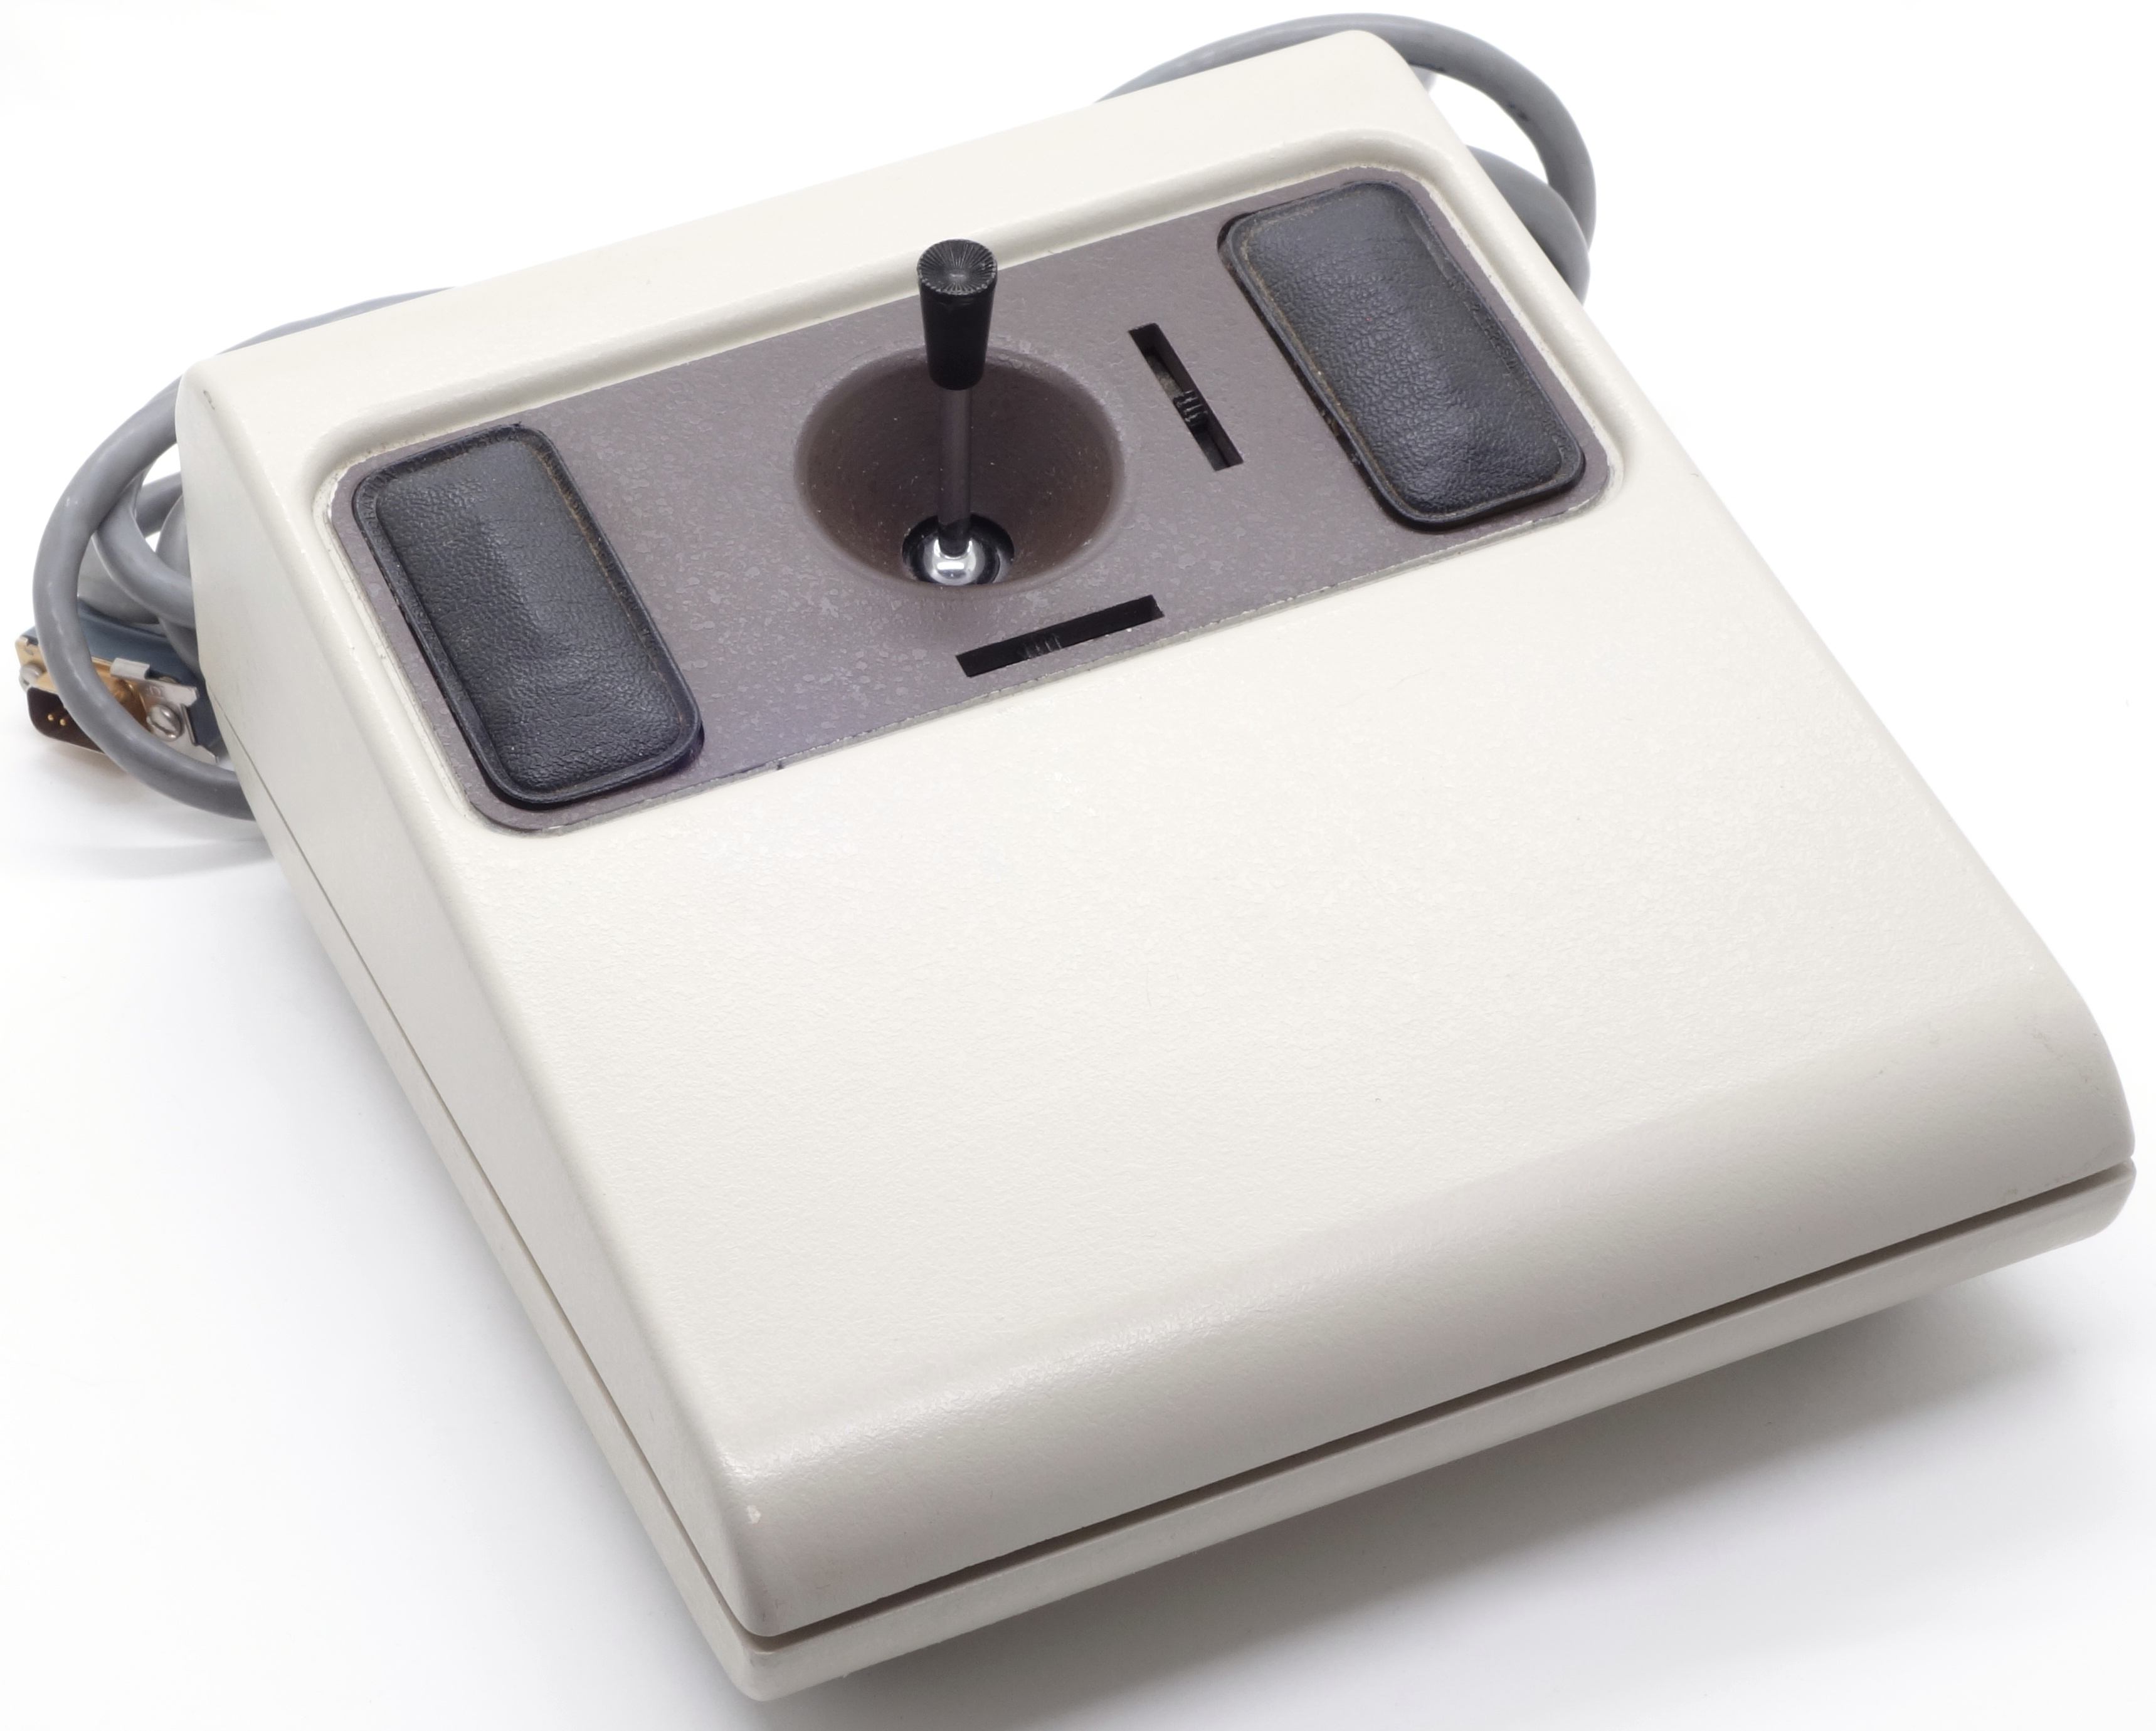
\includegraphics[scale=0.53]{1978_dec_h3060_joystick/pic_30.jpg}
    \caption{DEC H3060 joystick}
    \label{fig:DecJoystickPic}
\end{figure}

The joystick has four rubber feet and a beige plastic body. On the top side (fig. \ref{fig:DecJoystickTopAndBottom}) there is a metal plate that combines the controls: a small handle (the ``lever''), a pair of buttons on either side of it, and two trimmers. The buttons are called ``joystick interrupt switches'' by the manufacturer \cite{vsv11} and have an unusual design: an arc of rigid metal wire with a leather overlay \cite{joystick}.

\begin{figure}[h]
    \centering
    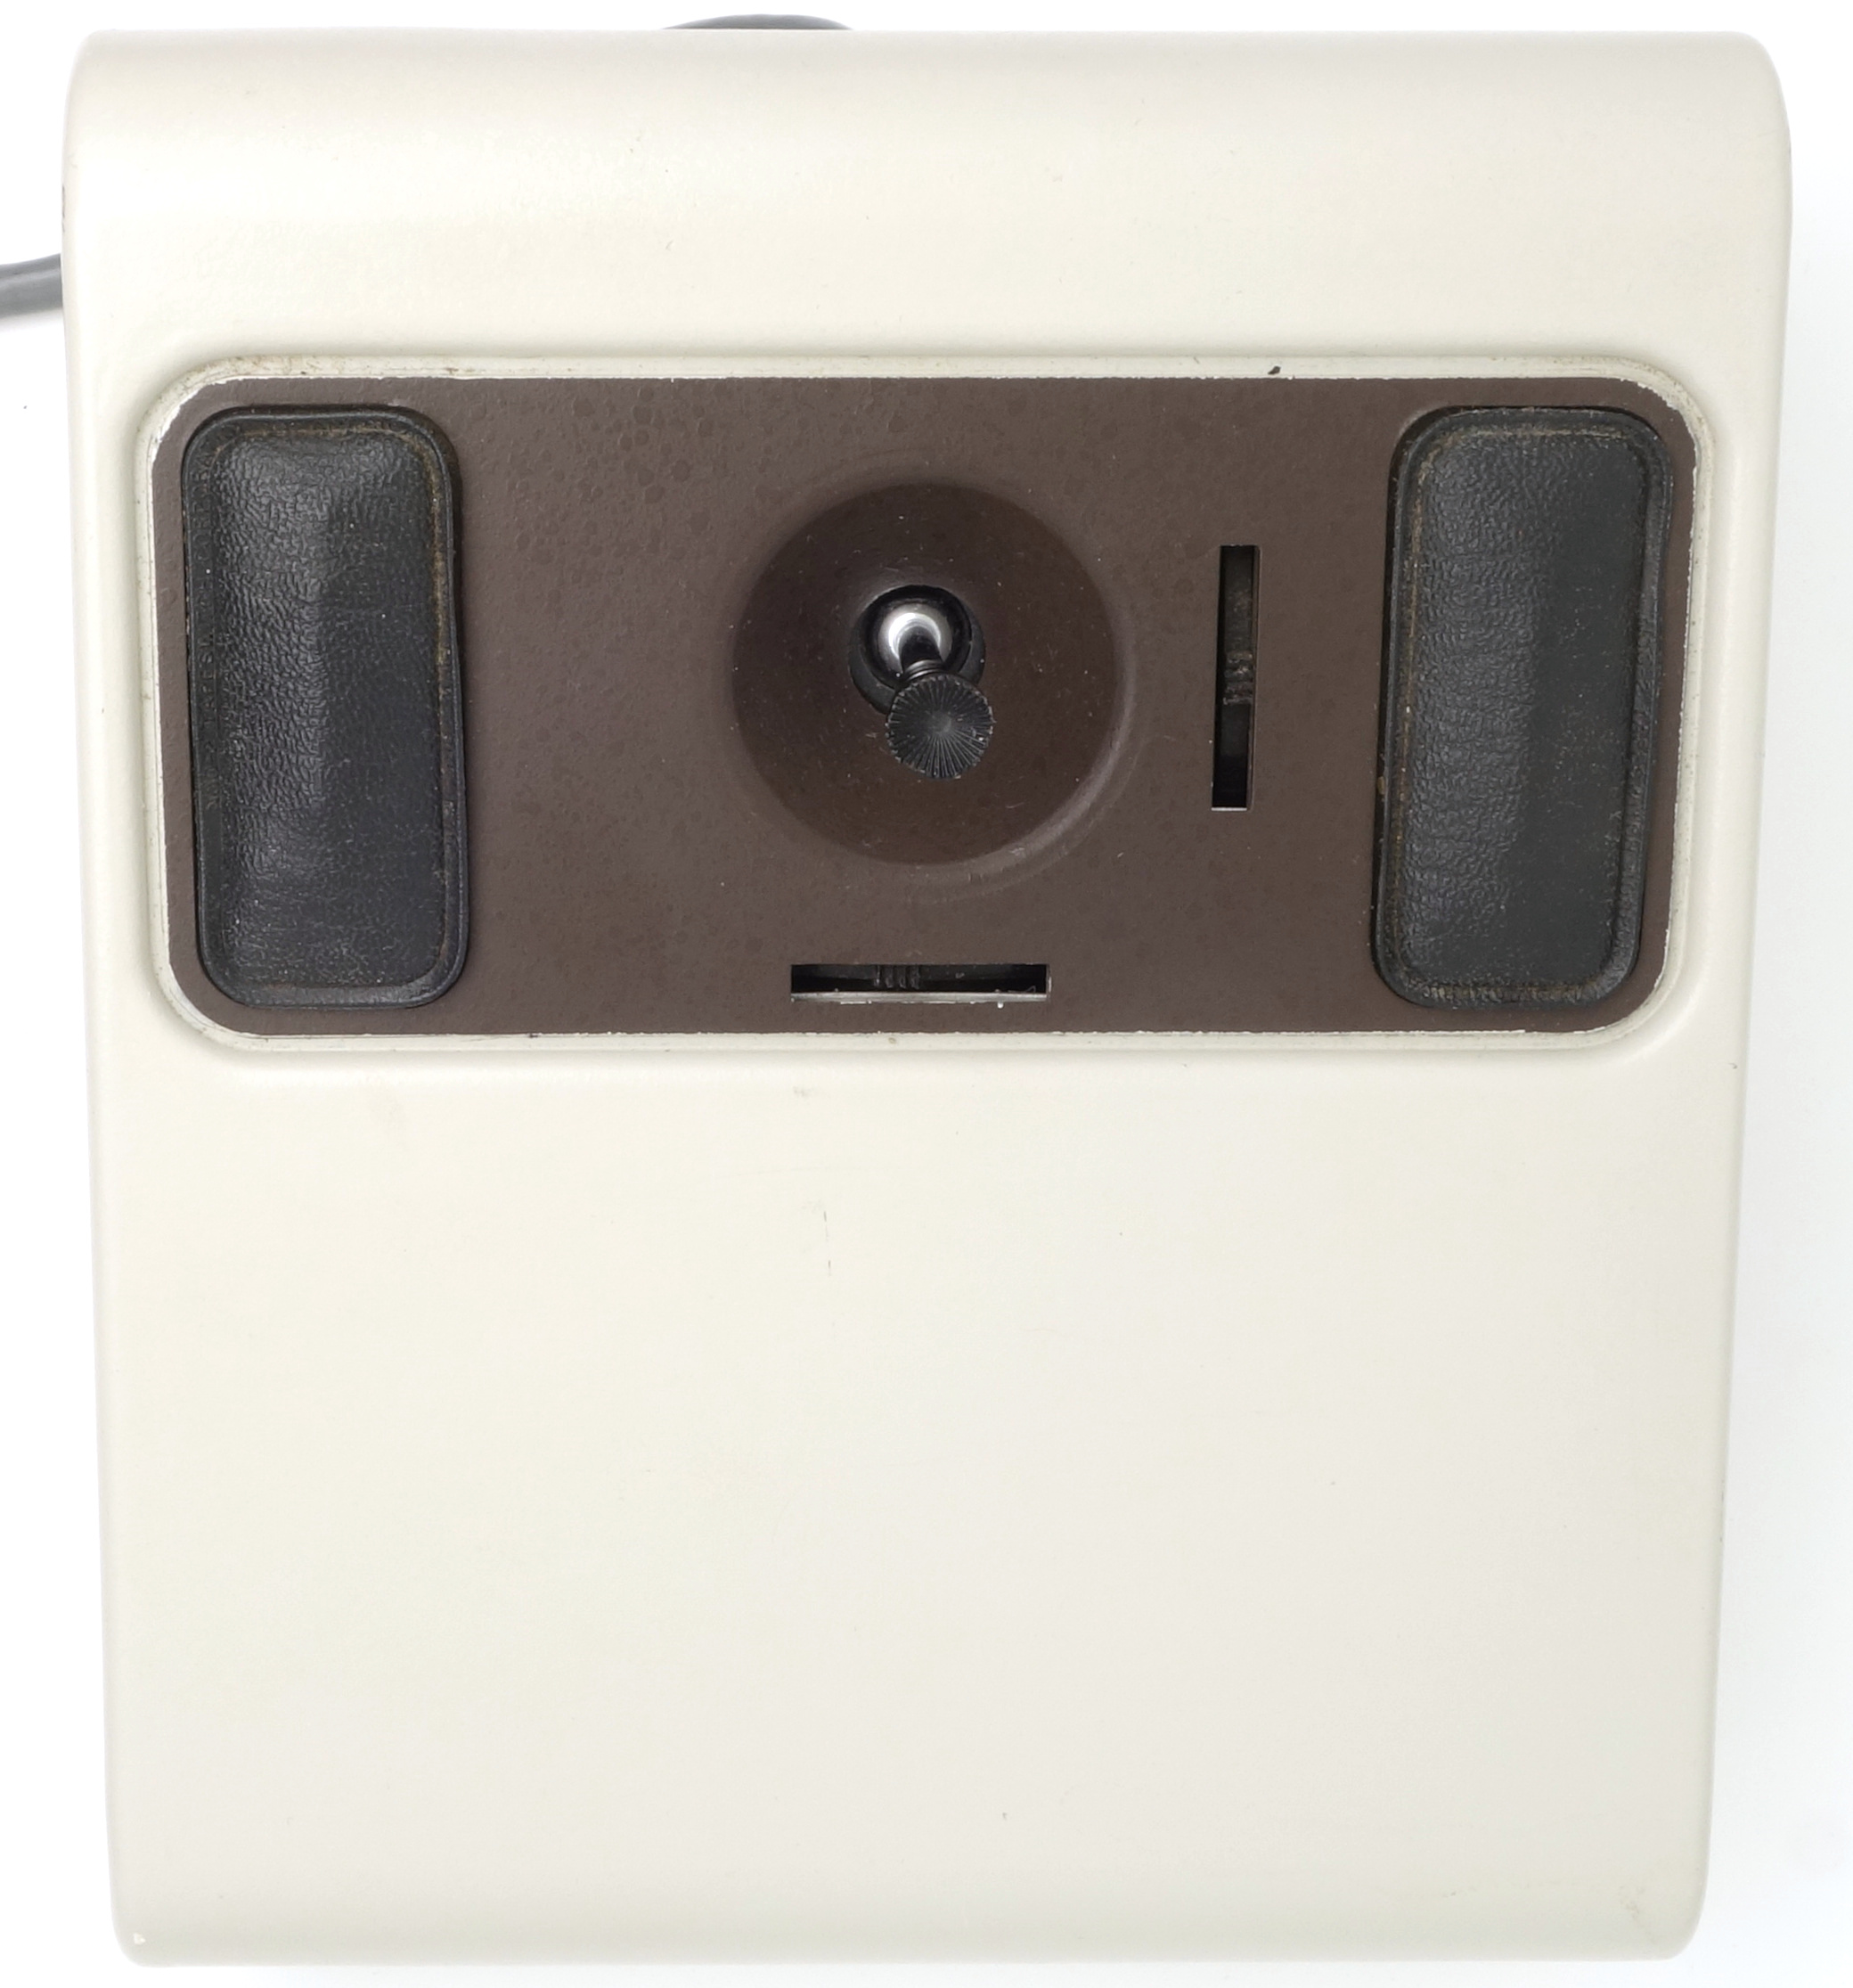
\includegraphics[scale=0.38]{1978_dec_h3060_joystick/top_15.jpg}
    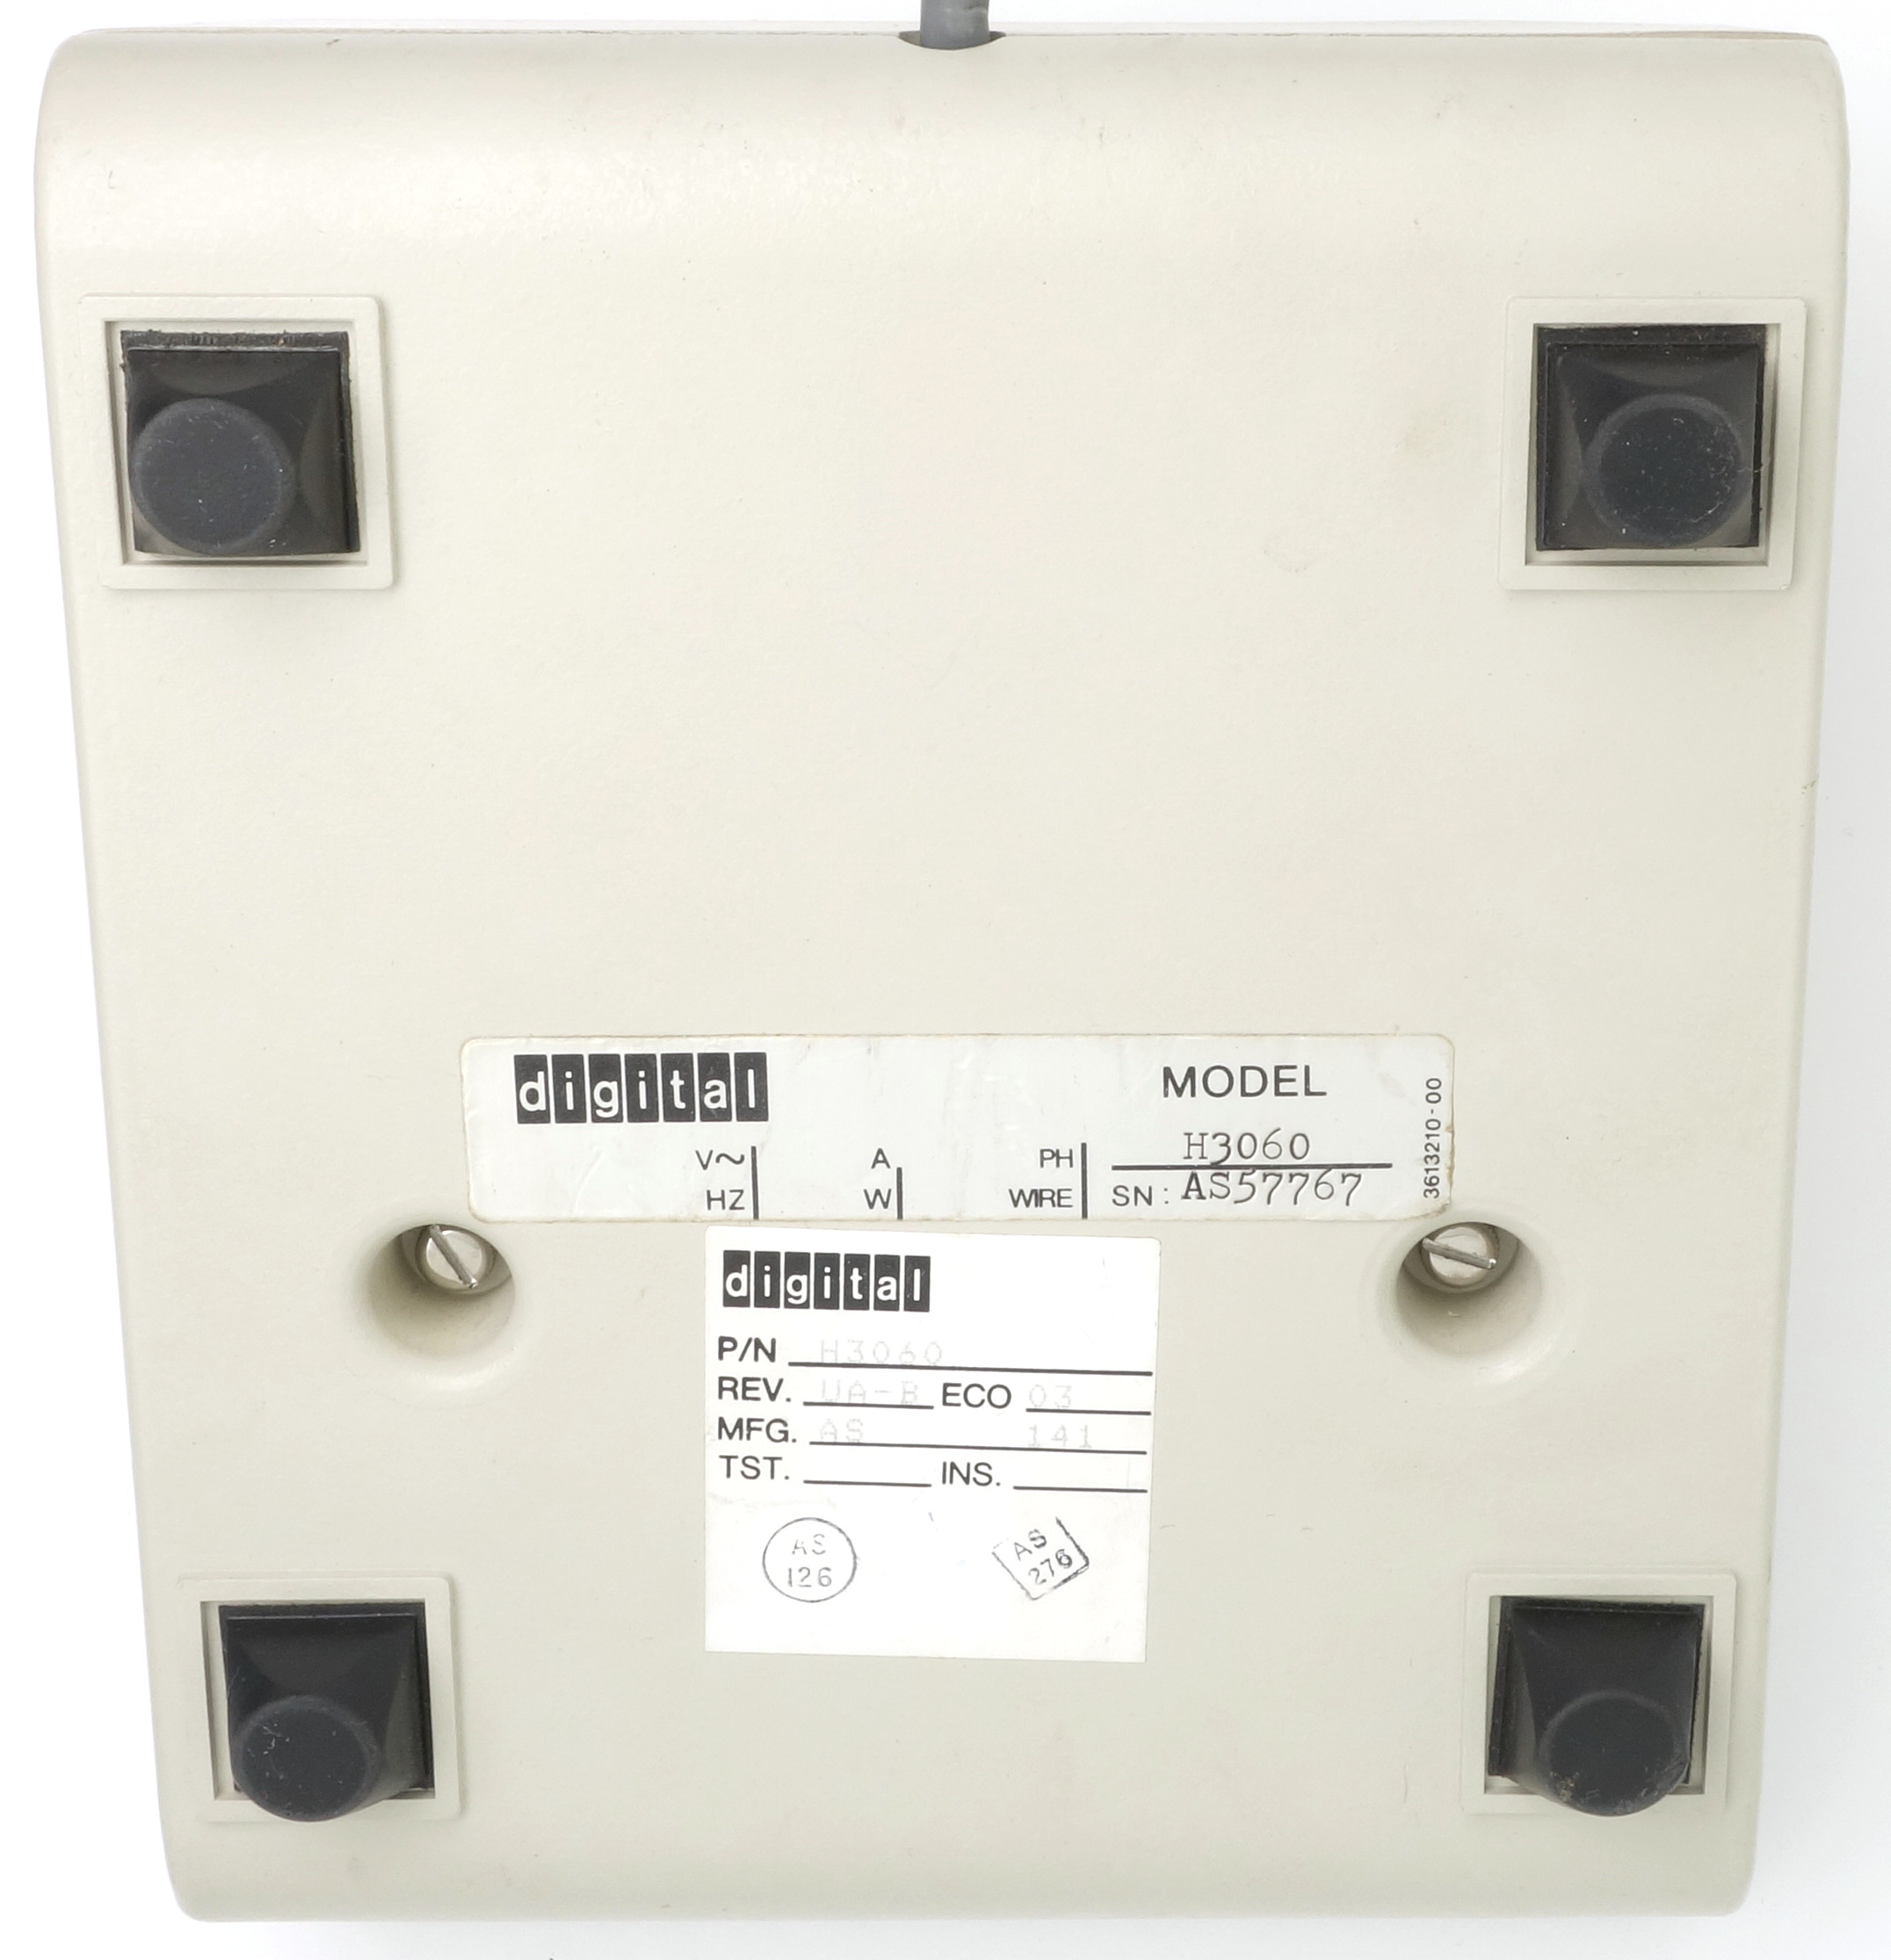
\includegraphics[scale=0.38]{1978_dec_h3060_joystick/bottom_15.jpg}
    \caption{DEC H3060 joystick, top and bottom views}
    \label{fig:DecJoystickTopAndBottom}
\end{figure}

The stick of the device is a standard unit: it can be found in models of other companies, for example in the Tektronix 4952 joystick, released on the market several years earlier. Unlike the stick, the device body is quite large (fig. \ref{fig:DecJoystickSize}) -- obviously for reasons of ergonomics and design, and not for placing electronic components.

It's comfortable enough to move the stick while holding it with fingers and resting your hand on the body (fig. \ref{fig:DecJoystickHand}). But the ``interrupt switches`` are a completely different story. Due to their construction, they are quite rigid, do not have a distinct movement and do not click when pressed. Therefore, it is difficult to measure the force when pressing them, and despite their elegant appearance, they represent one of the worst implementations of buttons in terms of ergonomics.

\begin{figure}[h]
    \centering
    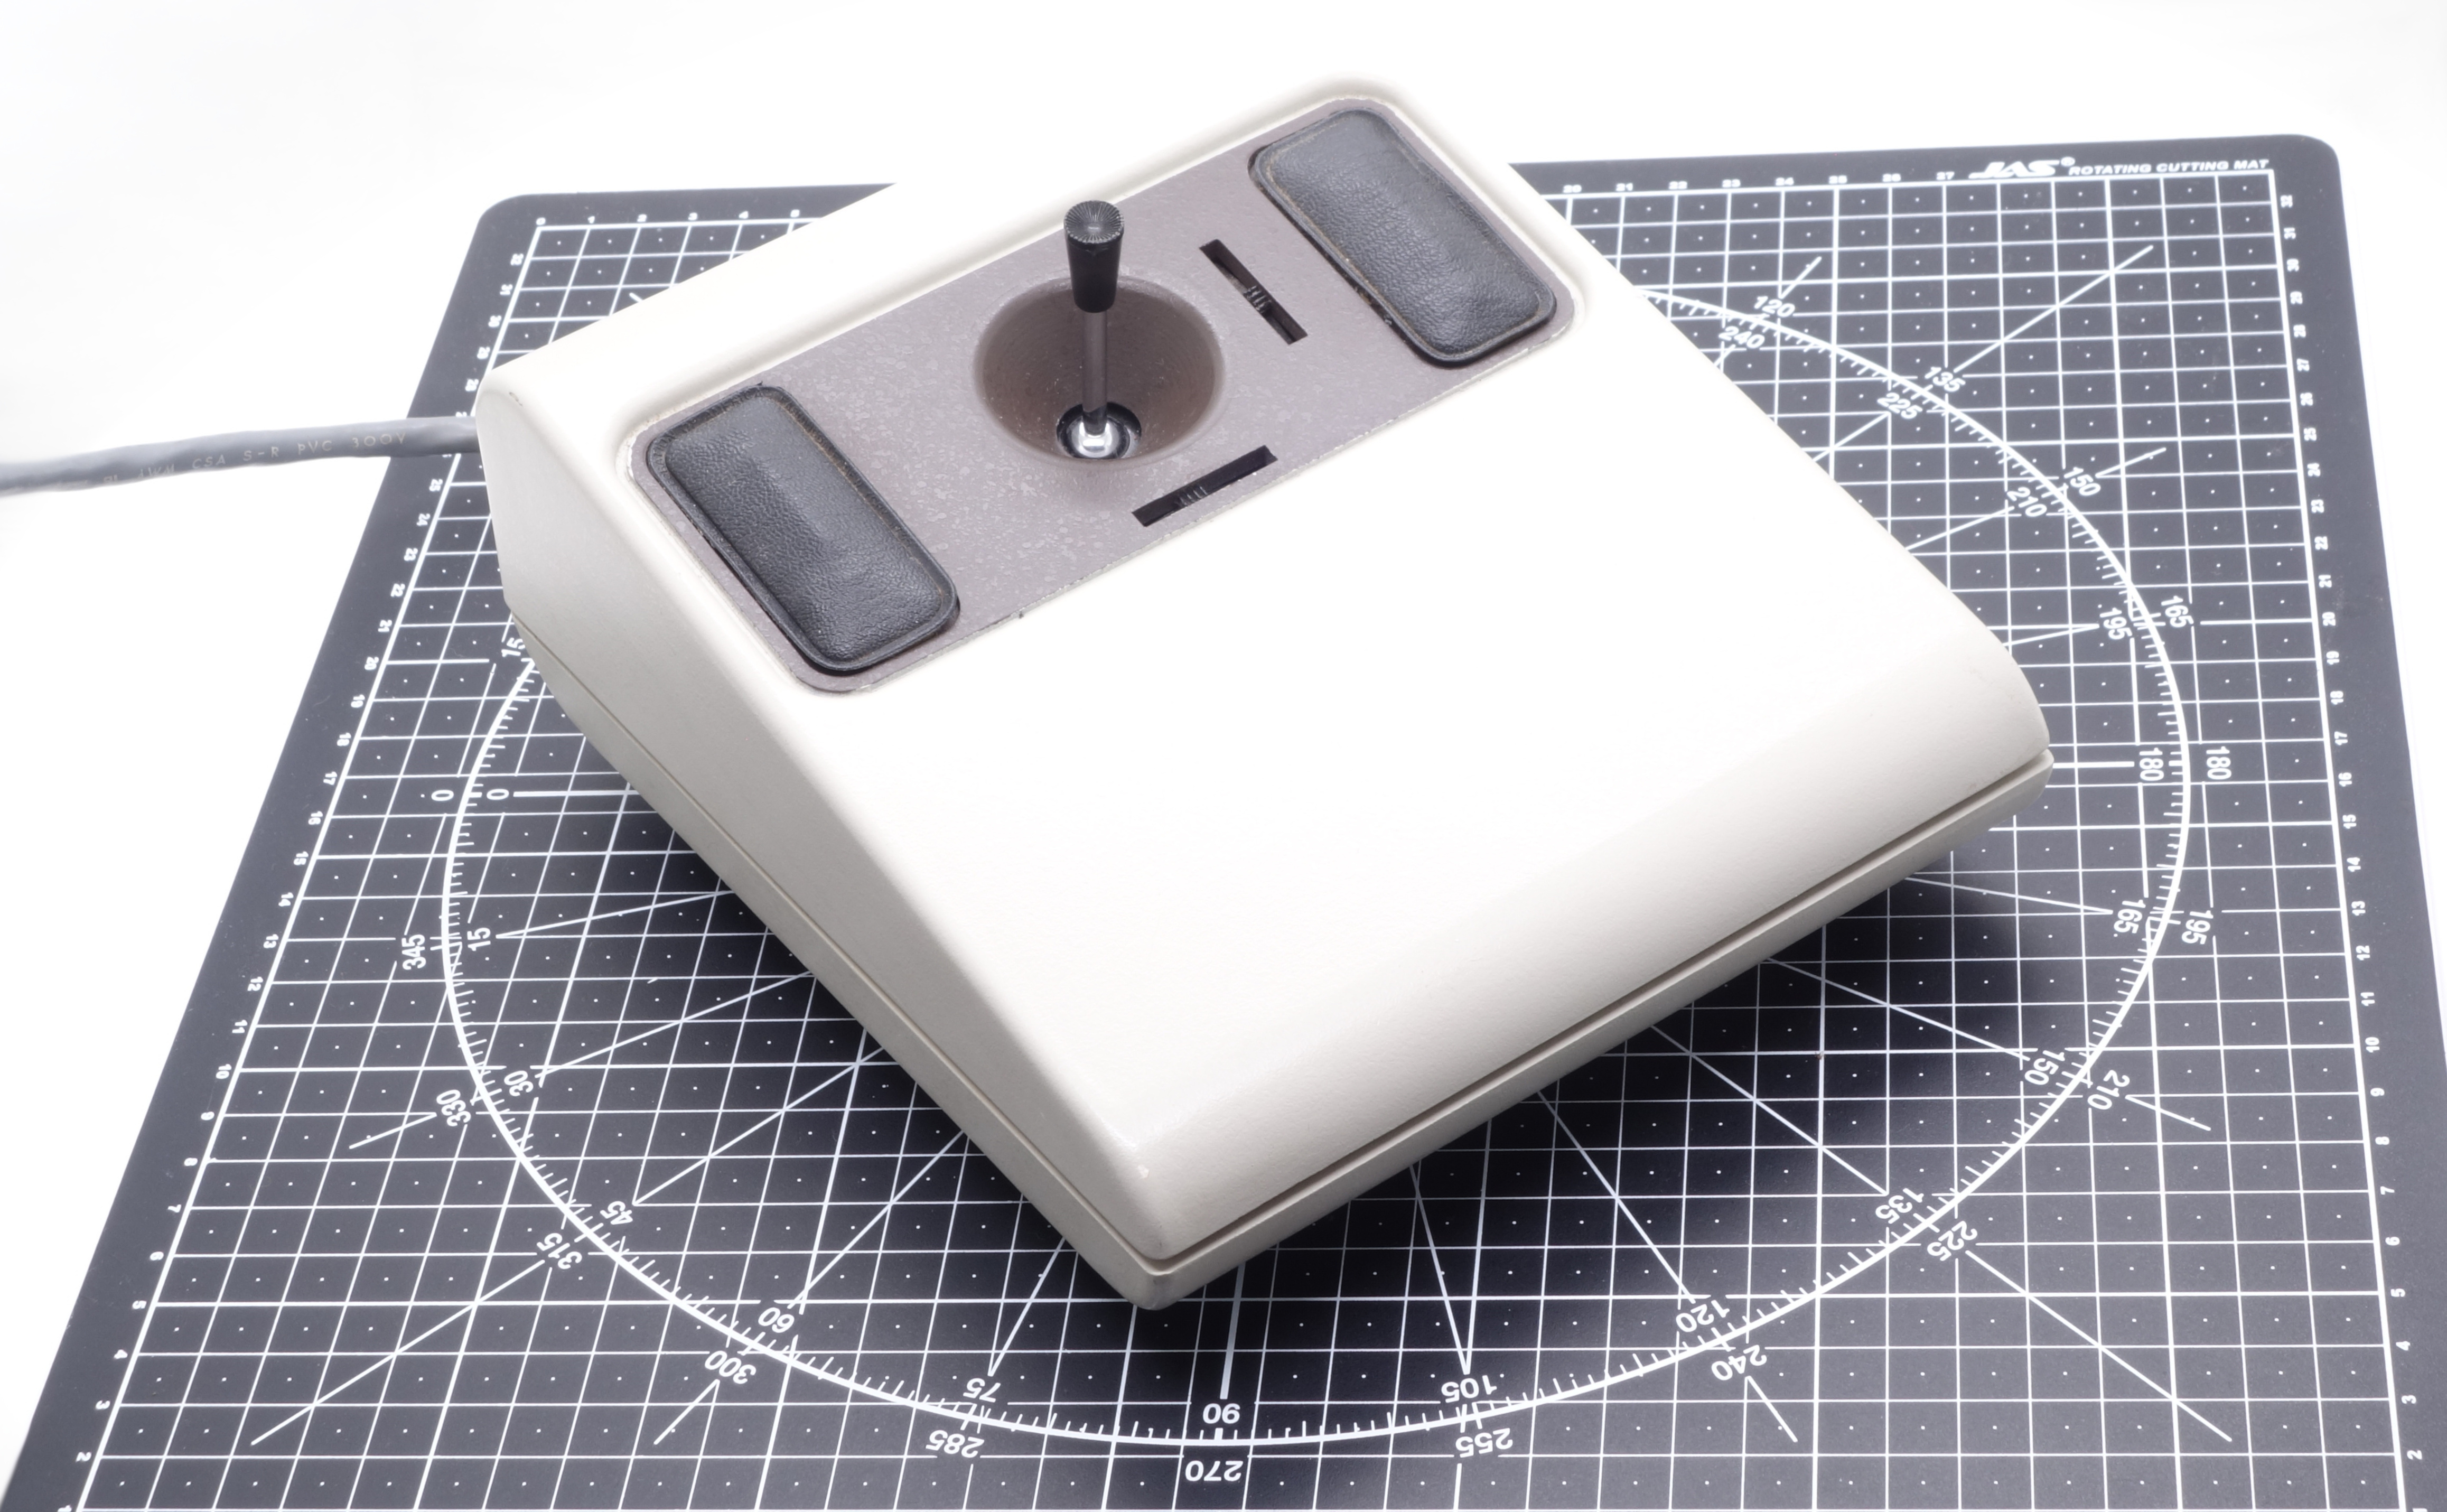
\includegraphics[scale=0.35]{1978_dec_h3060_joystick/size_30.jpg}
    \caption{DEC H3060 joystick on a graduated pad with a grid step of 1~cm}
    \label{fig:DecJoystickSize}
\end{figure}

The joystick buttons are connected in parallel and represent the same <<interrupt switch>>, which, depending on the situation, generates either a <<SWITCH>> interrupt (a signal of the button press to mark the desired position on the screen) or a <<CURSOR MATCH>> interrupt (selection of an object on the screen whose outline intersects with the cursor). In the last case the Display Processor stops executing the ``display file'' when the interrupt occurs, leaving the current position pointer to be read by software  \cite{vsv11}. This approach had originally appeared with vector displays and light pens and was later adapted for raster displays like the one of the VS11/VSV11 system.

\begin{figure}[h]
    \centering
    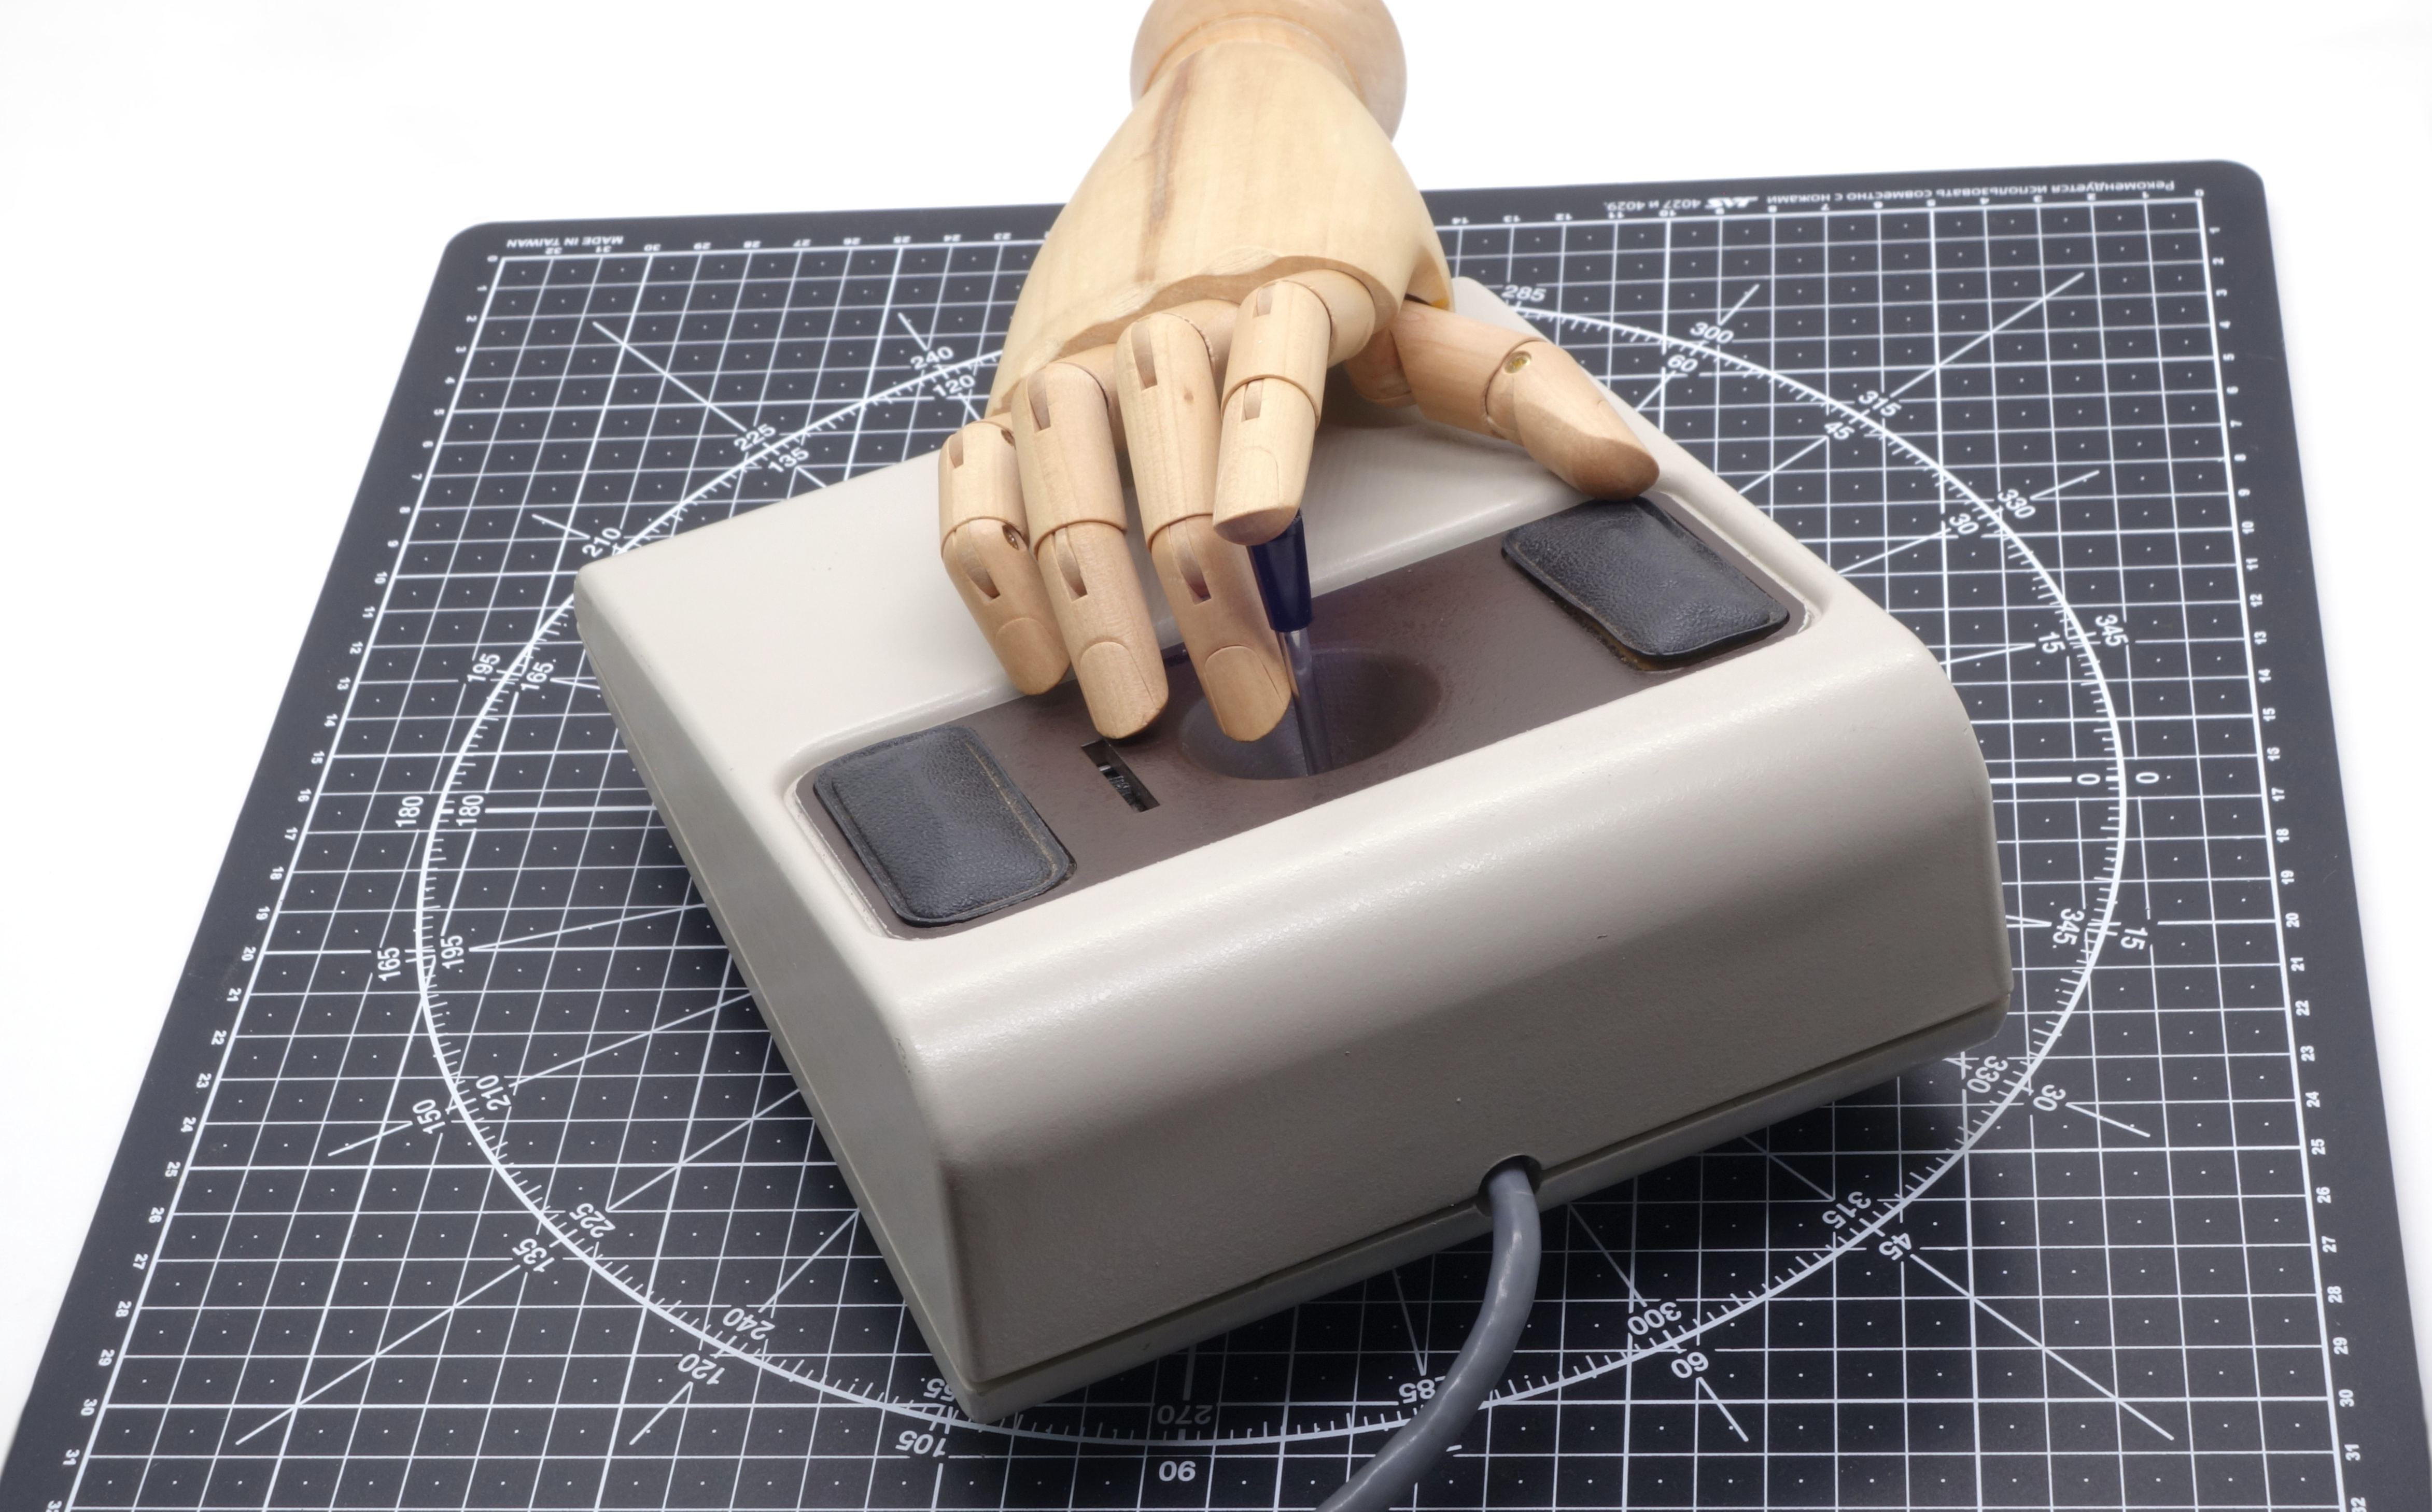
\includegraphics[scale=0.35]{1978_dec_h3060_joystick/hand_30.jpg}
    \caption{DEC H3060 joystick with a human hand model}
    \label{fig:DecJoystickHand}
\end{figure}

Stick tilt affects the cursor movement in a predictable way: direction of the movement is determined by the direction of tilt, while the tilt angle is proportional to the speed of movement. Drift tabs are used to adjust voltage to zero on $X$ and $Y$ outputs when the stick is in its vertical position.

So, the user was supposed to move the cross-hair cursor with the stick until it reaches specific point on a display, but the cursor can also be moved programmatically by writing into coordinate registers of the display processor.

Joystick was connected to the system using a long thick cable.

Disassembled joystick is shown in fig. \ref{fig:DecJoystickInside}. 

\begin{figure}[h]
    \centering
    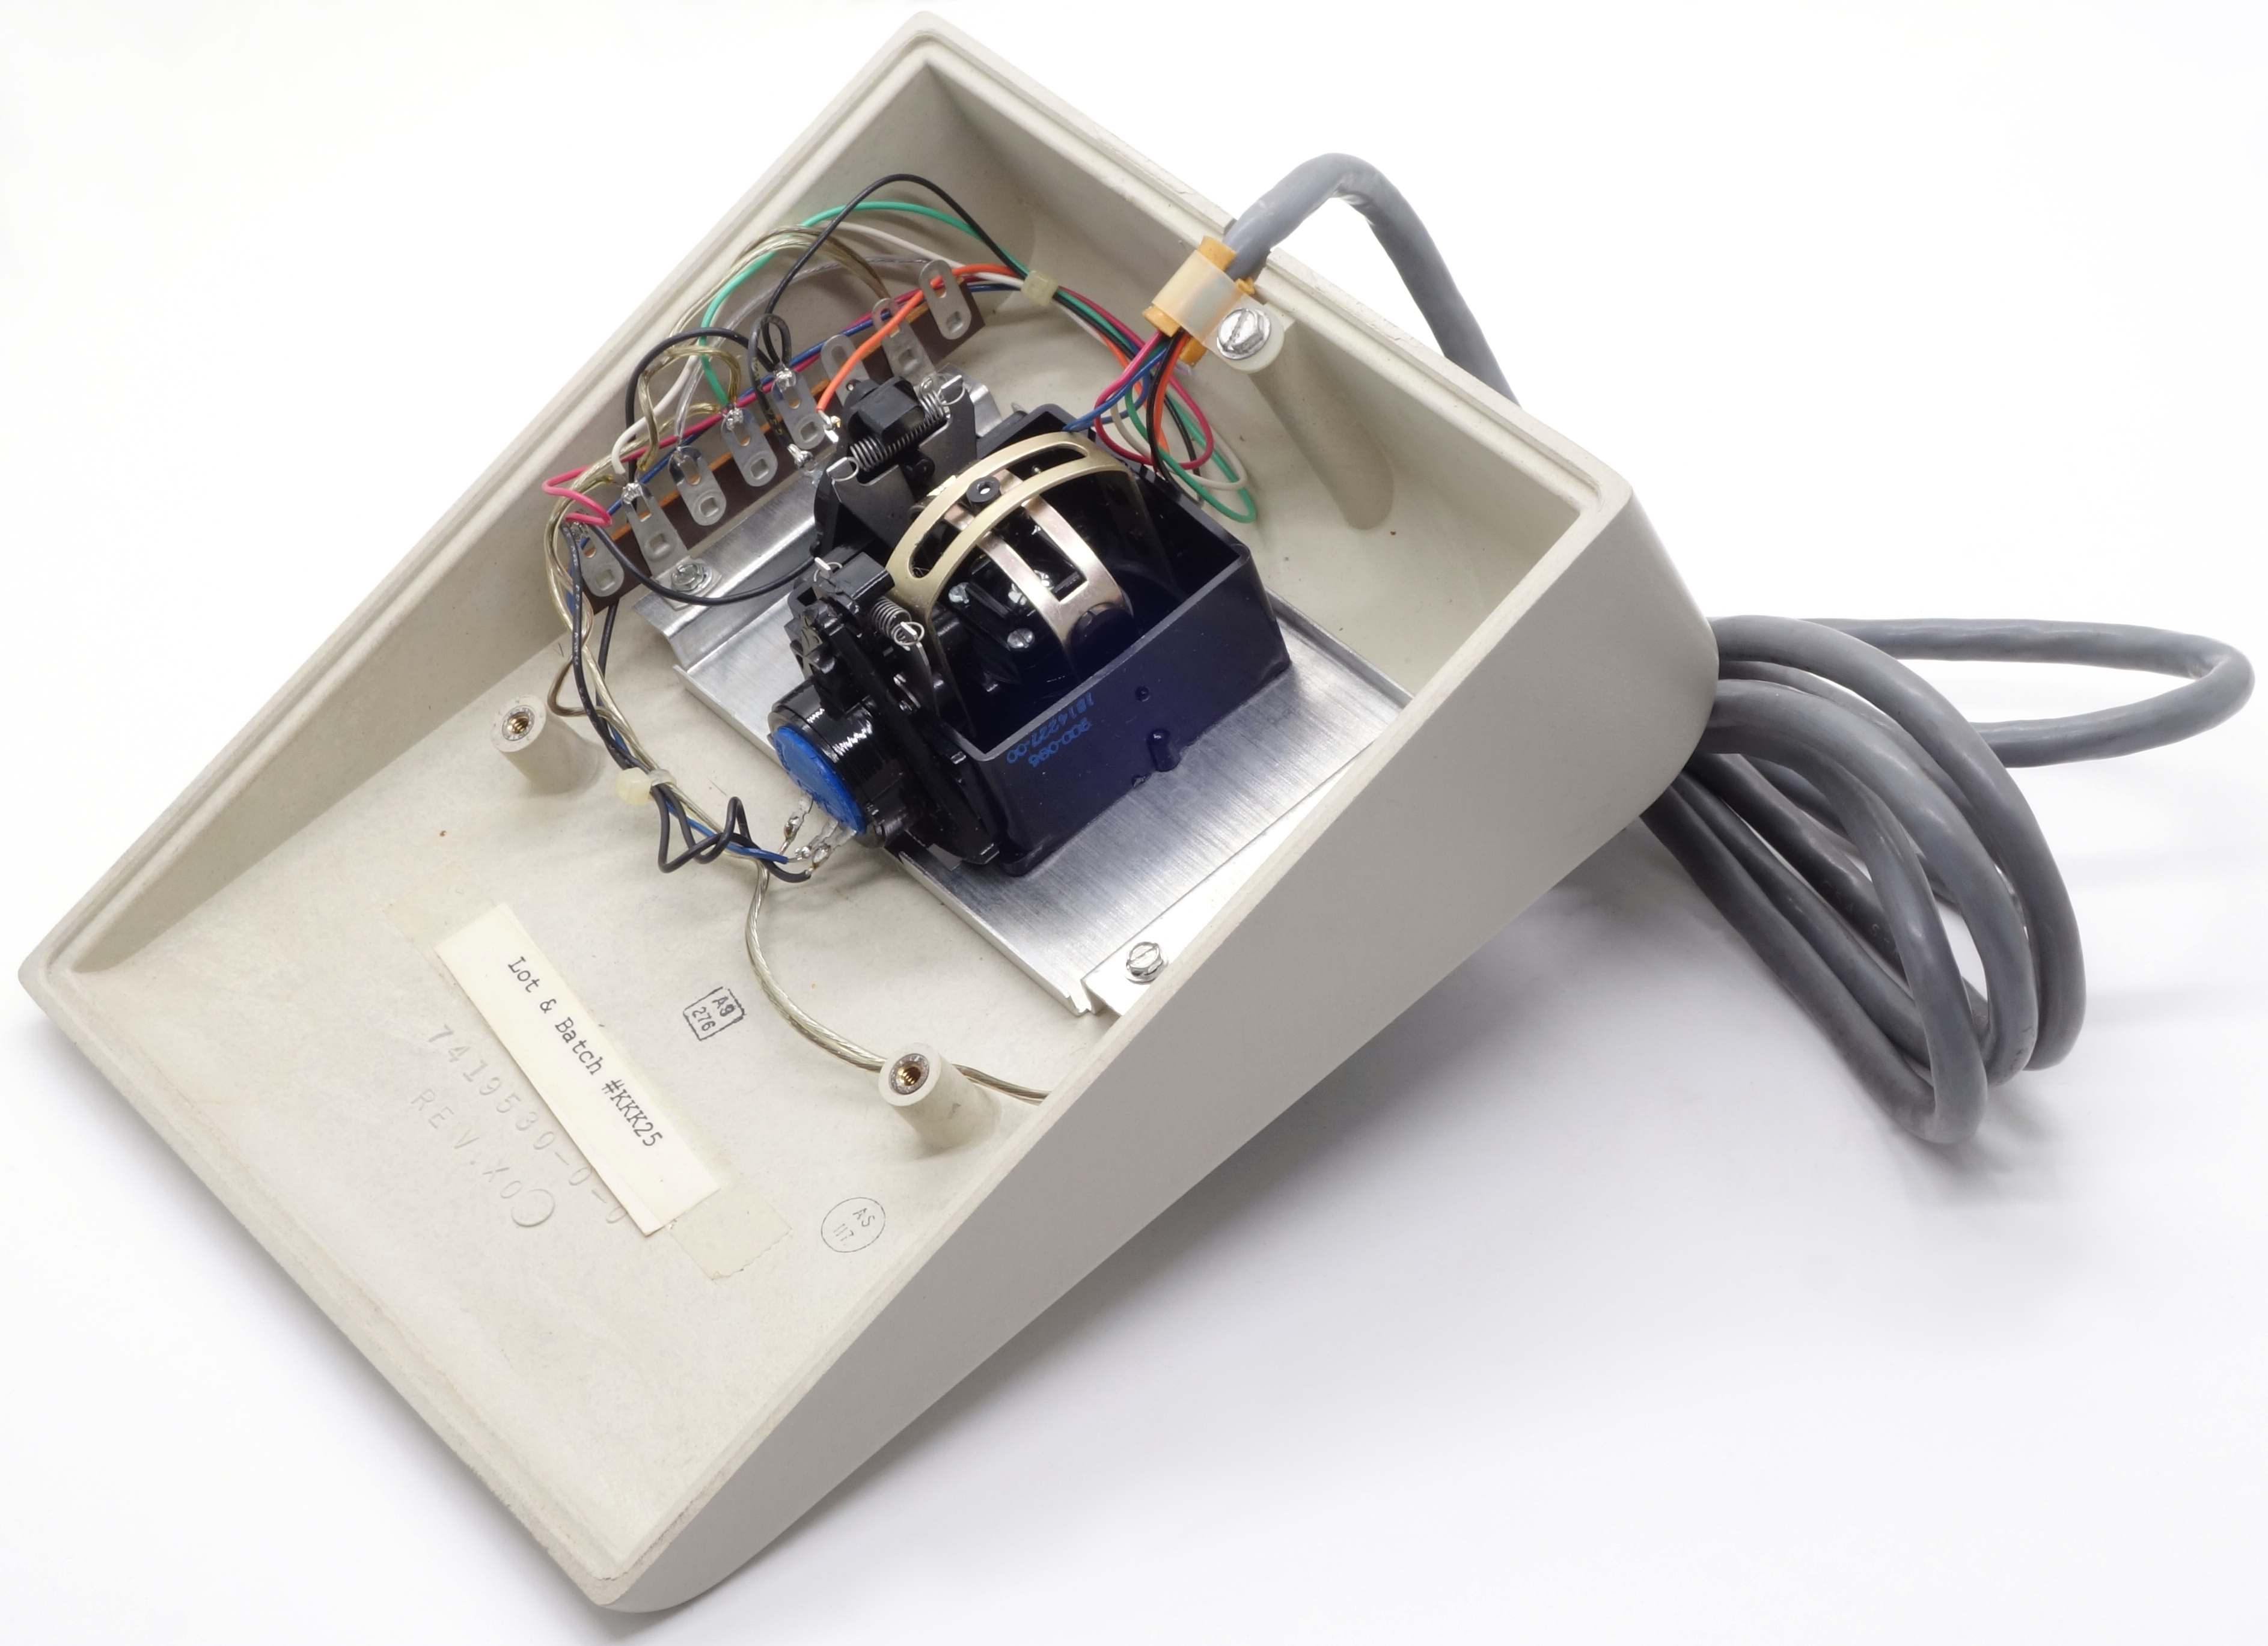
\includegraphics[scale=0.5]{1978_dec_h3060_joystick/inside_30.jpg}
    \caption{DEC H3060 joystick disassembled}
    \label{fig:DecJoystickInside}
\end{figure}

Trim tabs mechanically rotate the $X$ and $Y$ potentiometers to control drift.
The joystick assembly, including the stick and its mount, as well as potentiometers and coarse drift rotation tabs, is typical: it appears later unchanged up to complete interchangeability in a lot of analog joysticks produced for industrial needs.


\begin{thebibliography}{9}
\bibitem {joystick} VSV11 RASTER GRAPHICS SYSTEM. D\textbar I\textbar G\textbar I\textbar T\textbar A\textbar L CSS -- Computer Special Systems \url{https://www.pdp-11.nl/peripherals/comm/interface/vsv11/vsv11-info.html}
\bibitem {fiche} NCV-11 Diagnostic. DEC PDF-11 Diagnostic Program Listings. 1978. \url{bitsavers.informatik.uni-stuttgart.de/pdf/dec/pdp11/microfiche/Diagnostic_Program_Listings/Listings/CZNCCA0__NCV-11__DIAGNOSTIC__AH-E772A-MC__DEC_1978_bw.pdf}
\bibitem {flyer} VSV11 and VS11 Raster Graphics Systems. Digital Equipment Corporation. Jan 81 \url{https://ia804604.us.archive.org/17/items/TNM_VSV11_and_VS11_Raster_Graphics_Systems_-_digi_20171029_0045/TNM_VSV11_and_VS11_Raster_Graphics_Systems_-_digi_20171029_0045.pdf}
\bibitem{vsv11} VSV11/VS11 Raster Graphics System. Option Description. 1981. \url{https://archive.org/details/bitsavers_decgraphiconDescriptionDec81_14714530/mode/2up}
\end{thebibliography}
\end{document}
